\chapter{Bole volume\label{chap::bole_v}}
\begin{marginfigure}
	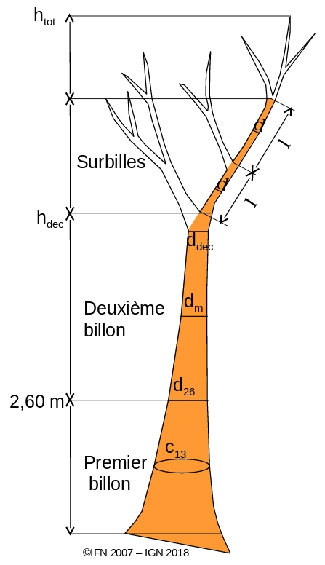
\includegraphics[width = \marginparwidth]{Figures/tree2.pdf}
	\caption{\label{fig::Vbole}}
\end{marginfigure}
The bole volume is considered the reference volume of the French \NFI{} and is computed via species-specific allometries. The formul\ae{} have changed over time, the most recent dating from 2016 \parencite{Morneau2016}. The allometric equations were fitted on the \NFI{} dataset, which contains the volumes of the butt log (from the stump to \qty{2.6}{\metre}), the second log (from \qty{2.6}{\metre} to \( \hdec \) --- defined in Tab. \ref{tab::notations}), and upper log sections if any (see Fig. \ref{fig::Vbole}). These three volumes rely on the circumferences at breast height, \qty{2.6}{\metre}, \( \hdec \), \( \ddec \), and the median diameter of the second log \( d_m \) and are derived using cylinder and Newton-Simpsons formul\ae{} \parencite{Gohon2024}. \\

In what follows, we sum up the equations currently used in the ``\nameref{sec::old_allom}'' section and compare them with new allometries recently developed \parencite{Gohon2024} in the section \nameref{sec::new_allom}. All the notations and definitions are gathered in Tab. \ref{tab::notations}.

\section{Two sets of equations\label{sec::old_allom}}

The annual living tree sample surveyed by the French \NFI{} is divided into two subsets:
\begin{description}
	\item [Complete trees] where girth (at breast height), \( c \), total height, \( h \), and taper height, \( \hdec \), are measured. These trees are randomly designated, ensuring that there is at least one individual per girth class, per species, and per plot.
	\item [Simplified trees] where only girth is measured.
\end{description}

For the so-called `complete trees', the bole volume is predicted using an allometric equation with three input variables (see equation \eqref{eq::fnew}), as described in \cite{Morneau2016}:
\begin{fullwidth}
	\begin{equation}
		\left\{
		\begin{aligned}
			\hat{V}_{\text{bole}} &= \frac{c^2 h}{4 \pi \left( 1 - \frac{1{,}3}{h} \right)^2} \hat f_{\text{new}} \\
			\hat f_{\text{new}} &= \left( \alpha + \beta c + \gamma \frac{\sqrt{c}}{h} + f(\hdec) + \delta \frac{1}{c^\epsilon} \right) \left[ 1 - b \left( \frac{0{,}07 \pi}{c} \right)^3 \left( 1 - \frac{1{,}3}{h} \right)^3 \right],
		\end{aligned}
		\right.
		\label{eq::fnew}
	\end{equation}
\end{fullwidth}
where \( f \) is a function of \( \hdec \) among the following:
\begin{alignat*}{2}
f(\hdec) & = f_{\text{max}}\!\left( \frac{\hdec}{\hdec + k} \right)^{1 + \rho} && \qquad f(\hdec) = \eta \ln\!\left( \frac{\hdec}{h} \right) \\
f(\hdec) & = \eta \ln(\hdec) && \qquad f(\hdec) = \eta \hdec
\end{alignat*}
The coefficients \( \alpha \) \dots, \( b \), and the function \( f \) are species-specific. Some of these coefficients also depend on the kind of terminal cut of the tree, either the stem top (\textit{regular cut}) or a sudden decrease in stem diameter (\textit{shape cut}). \\

For simplified trees, the bole volume is based on the predicted volume of a neighbouring complete tree. A one-variable allometric equation is used to adjust for the girth difference between the reference tree and the simplified tree when assigning bole volume.
\begin{tcolorbox}[breakable, title = Volume imputation]
We associate each simplified tree \( i \) with a complete tree \( j \) that belongs to the same plot, same species and same girth class and adjust the bole volume of \( i \) using a ratio relative to its reference tree:
	\begin{equation}
		\hat{V}_{\text{bole}}^{\text{imp}}(i) = \hat{V}_{\text{bole}}(j) \frac{V_{I}(i)}{V_{I}(j)},
		\label{eq::imputation}
	\end{equation}
	where \( \hat{V}_{\text{bole}} \) is the three variable equation \eqref{eq::fnew}, and \( V_{I} \) is a species-specific allometric equation that takes only \( c \) as an input variable (see equation \eqref{eq::allom_1}).
\end{tcolorbox}

Current one-variable allometric equations are built on log transformation:
\begin{fullwidth}
	\begin{equation}
		V_{I} = \exp \left[ \alpha + \beta \ln(c) + \gamma \ln(c)^2 + \delta \ln(c)^3 + \zeta \ln(c)^4 + \eta f(g) + \frac{\sigma^2}{2} \right],
		\label{eq::allom_1}
	\end{equation}
\end{fullwidth}
where \( f(g) \) is a function of local basal area. The coefficients \( \alpha \), \dots, \( \sigma \) depend on the tree species and contextual parameters (ecological area, altitude zone, property regime). 

\section{Motivations for changes}

Regarding the three-variable allometric equations (Eq. \eqref{eq::fnew}), the aim is to improve model parsimony so that future species models share the same formula and fitting no longer depends on the type of terminal cut. Also, a decision was made to no longer rely on the \( \hdec \) term for trees with regular cuts, since \( \hdec \) has not been measured for such trees since 2020 and must now be estimated using a third-party model. This is achieved by defining \( \hdec' \) as:
\[
	\hdec' =
	\begin{cases}
		\hdec & \text{in case of a shape cut} \\
		h & \text{otherwise}
	\end{cases}
\]

For monitoring stock variations over time, the new coming inventory method will assess tree sample data twice. Tree samples are surveyed a second time, but only tree girth is measured again. So, one-variable allometric equations shall be used to assess tree new volume at second survey given old and new girth, the same way than simplified trees (see \ref{eq::imputation}). For that purpose, one-variable volume equations have to be an increasing function of girth. In particular, an explanatory variable \( f(g) \) involving local basal area, conveying stand competition, has to be questioned.  

The approach of new allometric equations development is detailed in \cite{Gohon2024}.  

\section{New bole models\label{sec::new_allom}}

Like current equations, future three-variable models are fitted using French NFI data (see \ref{chap::def} 3.). It models a shape coefficient \( f_{\text{new}} \) (see \ref{eq::fnew}) an analogous way than \cite{Morneau2016}.  

\[
	\hat f_{\text{new}} = \alpha + \beta c + \gamma \frac{\sqrt{c}}{\hdec'} + \delta \frac{\sqrt{\hdec'}}{c^2 h} + \eta \left( 1 - \frac{\hdec'}{h} \right)
\]
where coefficients (\( \alpha \), \( \beta \), \( \gamma \), \( \delta \), \( \eta \)) only depend on the tree species.  

New single-variable models are fitted to volume estimates of complete trees from recent inventory campaigns.

\[
	V_{I} = \mathrm{e}^{\alpha + \beta \ln(c) + \gamma \ln(c)^2 + \frac{\sigma^2}{2}},
\]
where (\( \alpha \), \( \beta \), \( \gamma \), \( \sigma \)) still depend on the tree species and on the same contextual parameters (ecological area, altitude zone, property regime).

New and current models perform similarly.
Survey estimates (see for instance \ref{fig::estimate_vbole_bygirth} and \ref{fig::estimate_vbole} from \cite{Gohon2024}) are a go-to output to foresee the forthcoming effect of new allometric equations on \NFI{} results. It shows lower volume estimates for small trees and slightly higher volume estimates for bigger trees, and consequently higher volume growth estimates. Differences never exceed confidence intervals.

\begin{figure}[h]
	\centering
	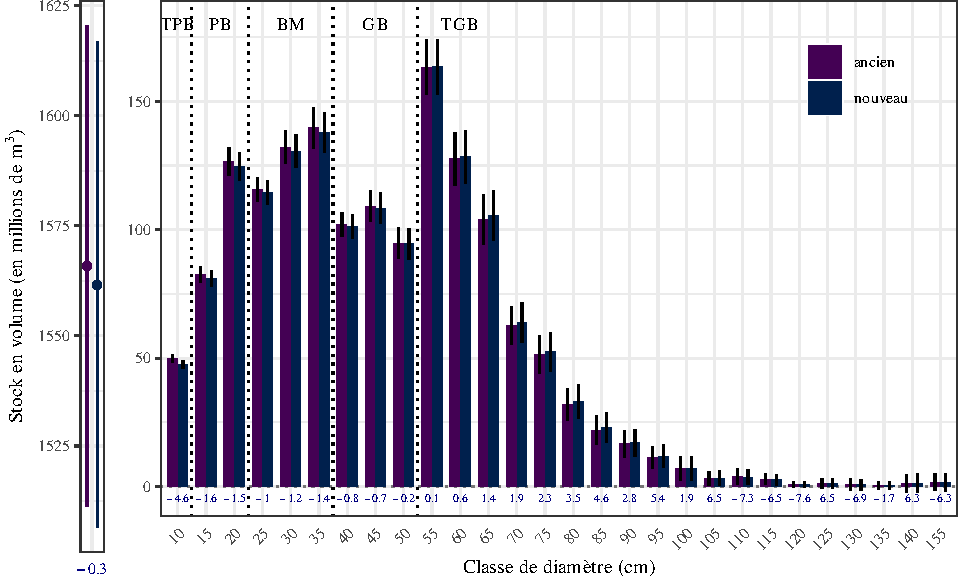
\includegraphics[scale = 0.6]{Figures/estimate_vbole_bygirth.pdf}
	\caption{National bole volume estimates for trees with height measures, by rounded girth. \label{fig::estimate_vbole_bygirth}}
\end{figure}

\begin{figure}[h]
	\centering
	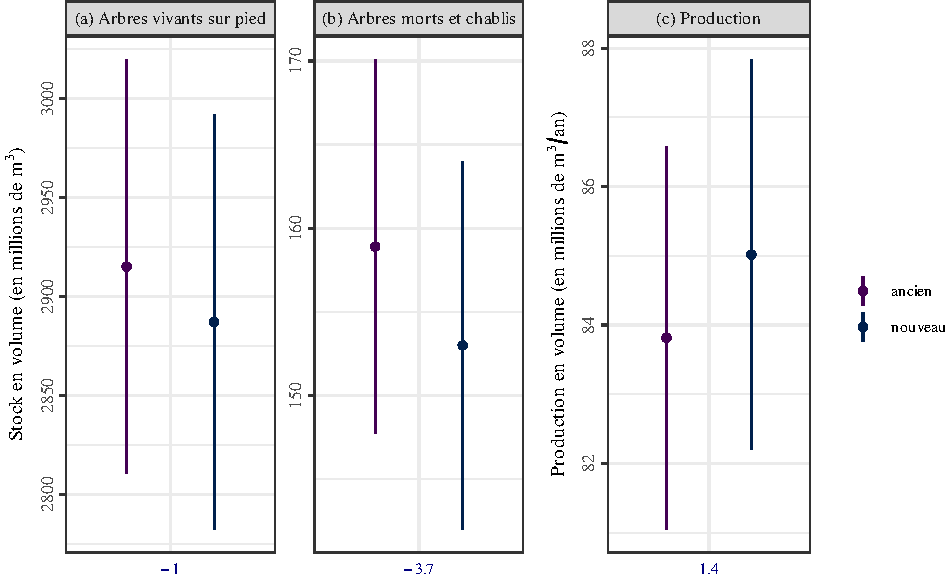
\includegraphics[scale = 0.6]{Figures/estimate_vbole.pdf}
	\caption{National bole volume and growth estimates for all living trees and dead trees. \label{fig::estimate_vbole}}
\end{figure}
